\begin{frame}{Research plans: Problems}
    \begin{itemize}
        \item How could complex network theory make it better for urban life?
        \item Dig in complex network, especially structural and temporal heterogeneities of the contact network.
        \item Feeding back: what does space mean for complex networks?
    \end{itemize}
\end{frame}
\subsection{Physics and society}
\begin{frame}{Physics and society}
E.g., how can we interpret and improve \textit{urban traffic networks} through statistical physics?
    \begin{itemize}
        \item The benefits of public transport\cite{buchanan2019benefits}, $T/P = 1-p$
        \item Topology and the spatial evolution of neighborhoods v.s. slums in cities\cite{brelsford2018toward}
        \item Urbanization correlated to hantavirus epidemics
    \end{itemize}
    \begin{figure}
        \centering
        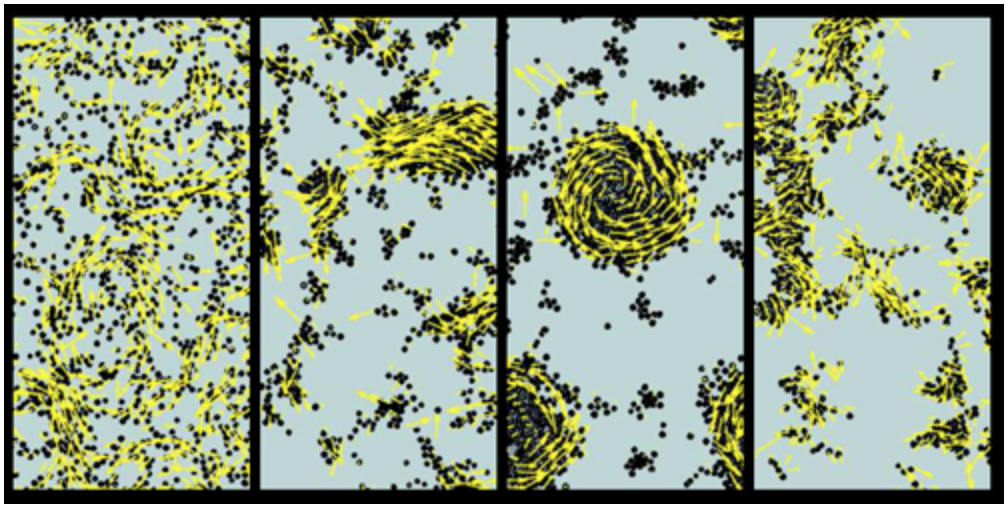
\includegraphics[width = 0.6\linewidth]{Pics/rwprl.png}
        \caption{Collective Dynamics of microbial. H. Karani et al., Phys. Rev. Lett. (2019)}
        \label{fig:rwprl}
    \end{figure}
\end{frame}

\begin{frame}{Physics and society}
    A design for road network generation towards cities without slums: 
    \begin{itemize}
        \item Based on the generation method in \cite{PhysRevLett.100.138702} with different optimization purpose: from \textit{connecting to the network the still unconnected centers using as little as possible road length}, to \textit{a linear combination of connectivity and tendency to get a block surrounded by roads}.
    \end{itemize}
    \begin{figure}
        \centering
        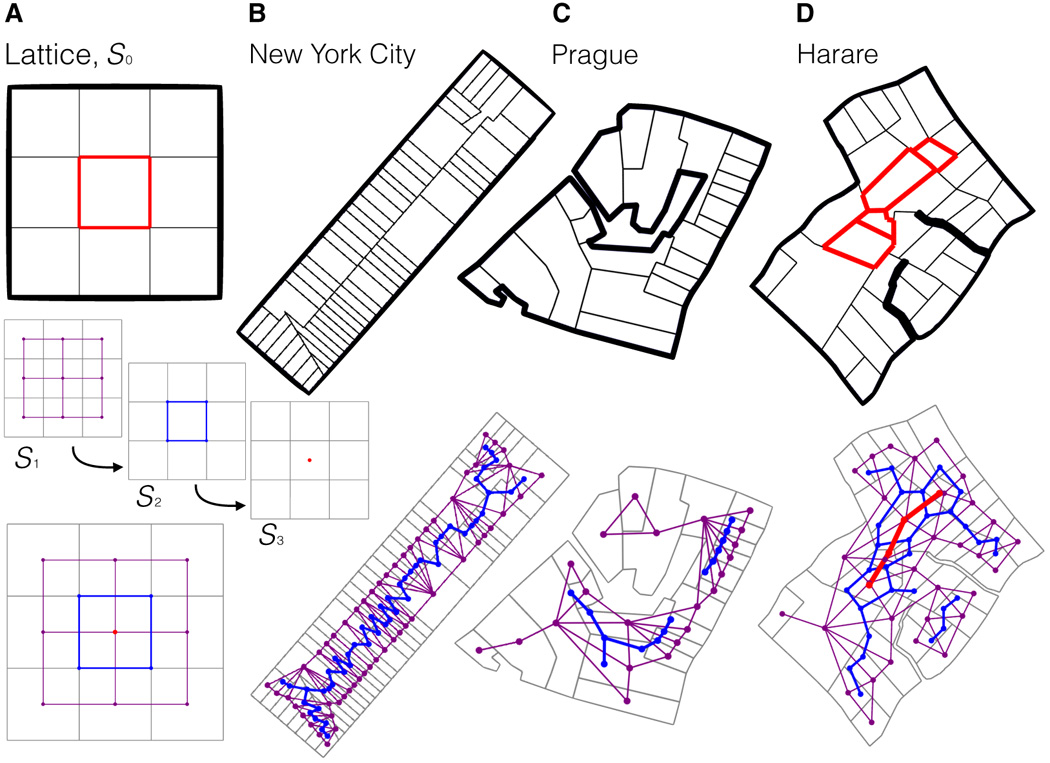
\includegraphics[width = 0.45\linewidth]{Pics/F1.large.jpg}
        \caption{Towards cities without slums, \cite{brelsford2018toward}}
        \label{fig:withoutslum}
    \end{figure}
\end{frame}

\subsection{Structures}
\begin{frame}{Structures in complex systems}
\begin{itemize}
    \item Predictability\cite{sun2020revealing,scarpino2019predictability} through \textit{compression of graphical structures} or \textit{permutation entropy}.
    \item Controllability\cite{liu2011controllability,gao2014target,angulo2019theoretical}
    \item Minimum of complex network\cite{barzel2015constructing}
    \item Geometric renormalization for the growth of modular networks\cite{song2006origins}
    \item ......
    \begin{figure}
        \centering
        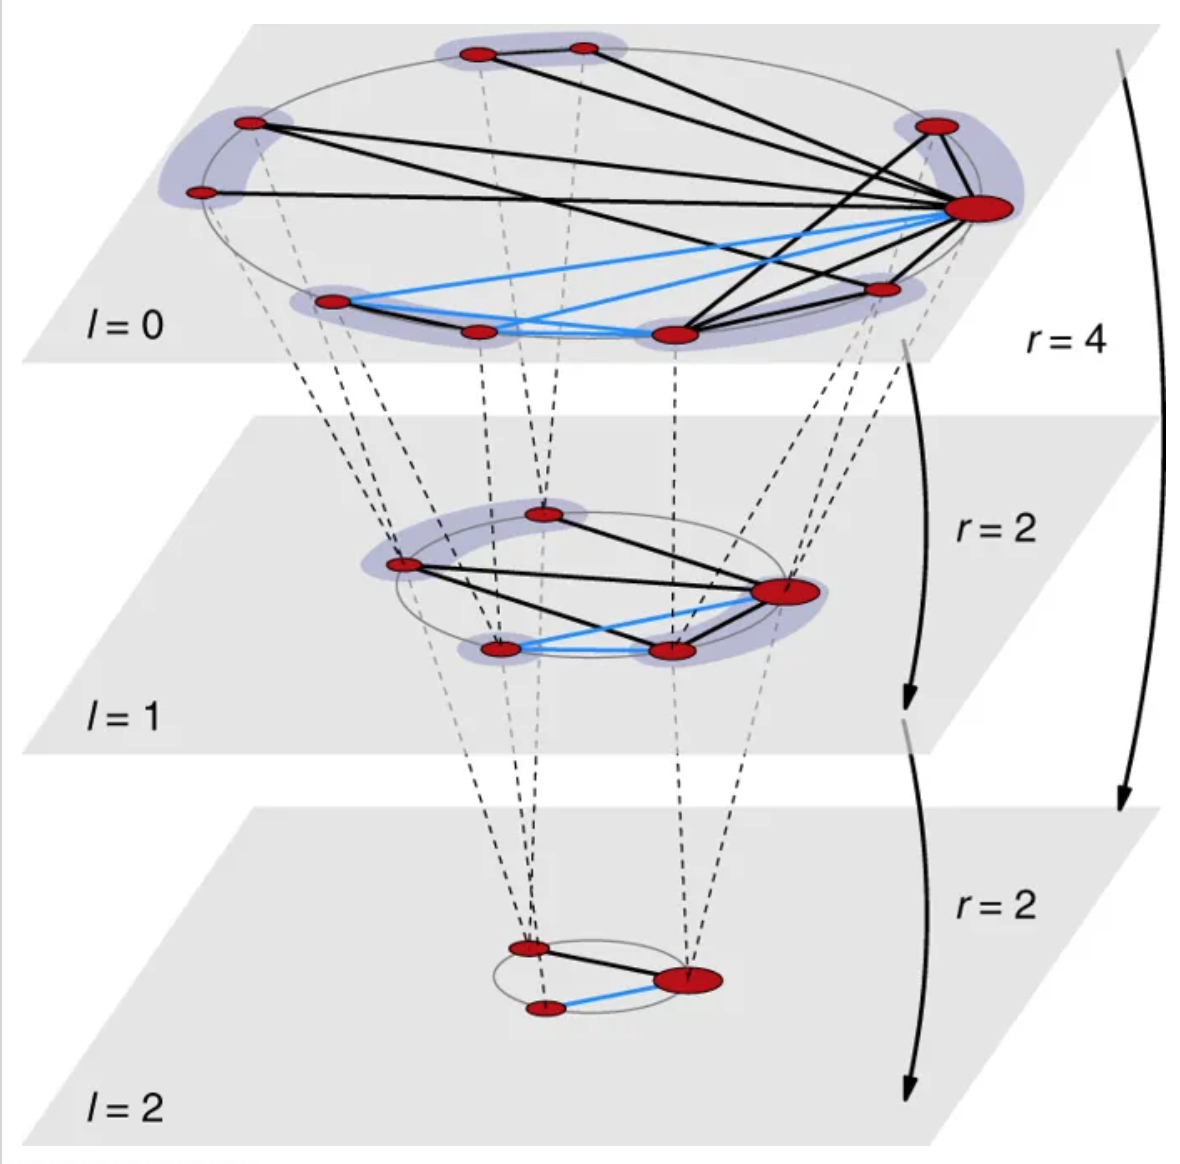
\includegraphics[width = 0.4\linewidth]{Pics/gr.png}
        \caption{Structural transitions of network by renormalizaiton group. From Ref.\cite{garcia2018multiscale}}
        \label{fig:my_label}
    \end{figure}
\end{itemize}
    
\end{frame}

\subsection{Feeding back}

\begin{frame}{Feeding back: What can those beyond links tell network?}

\begin{itemize}
    \item Density-based analysis: carbon emission, spatial structures, anomalous structures(tumors)...
    \item The variations of controllability of network is non-linear...
    \item Spatial networks, represented by epidemic models, are now highly related to human mobility models, as a preface of Physical Review E:
    \begin{figure}
        \centering
        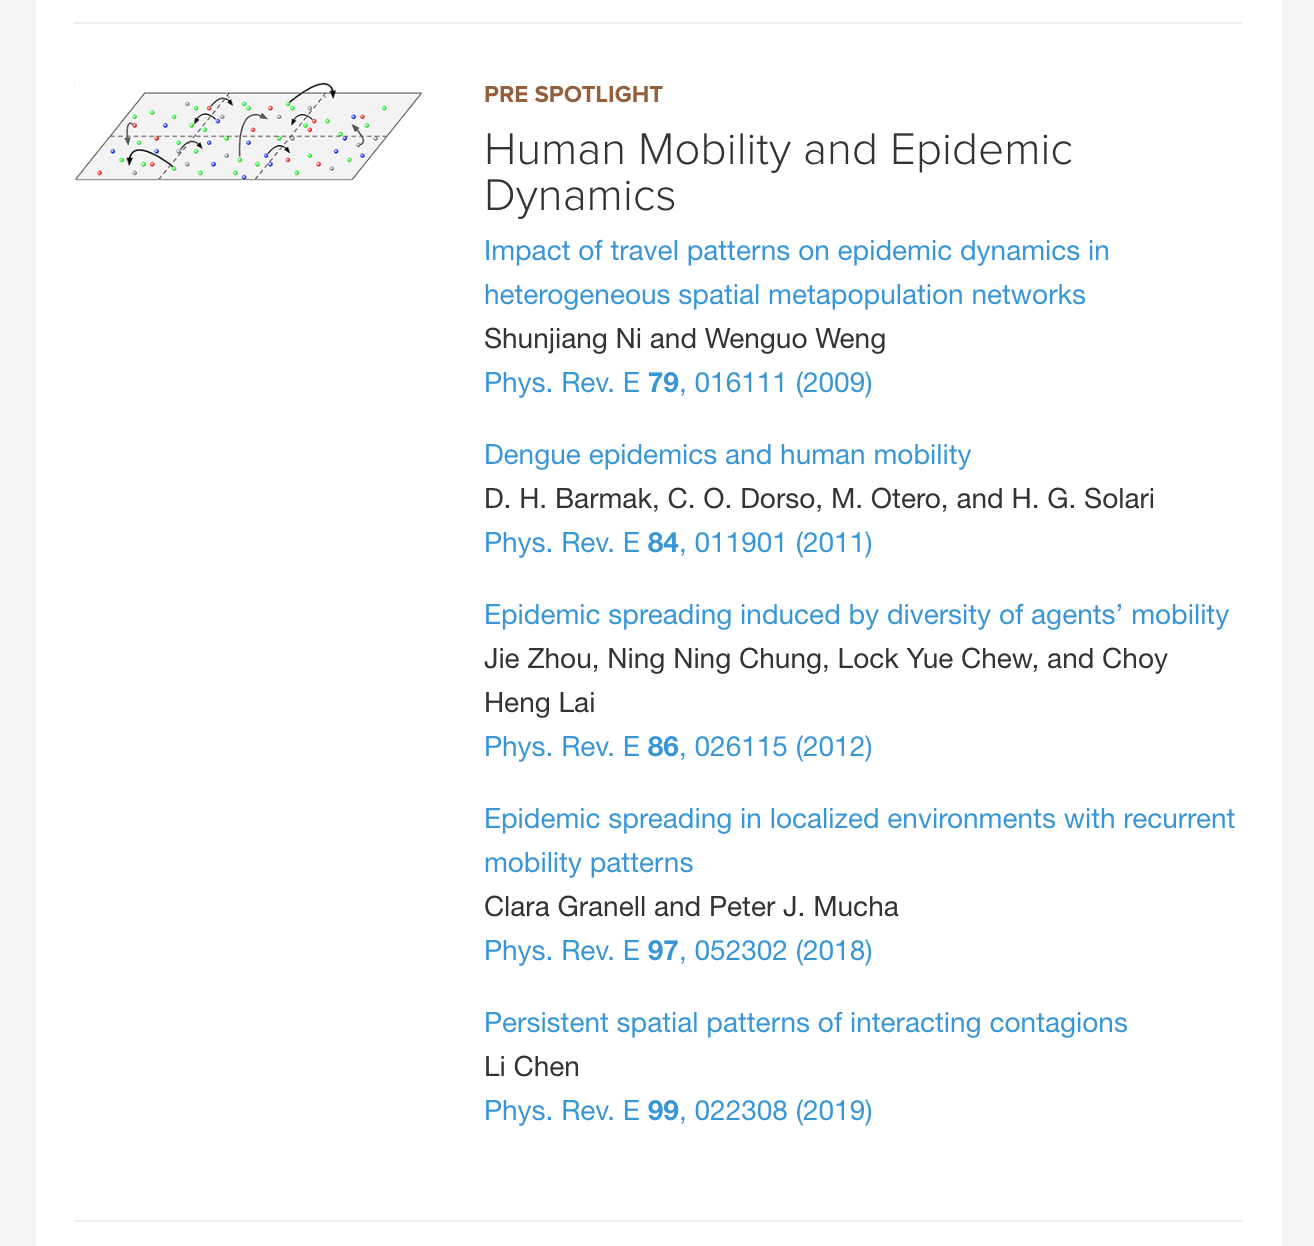
\includegraphics[width = 0.5\linewidth]{Pics/preface.png}
    \end{figure}
\end{itemize}
    
\end{frame}

\begin{frame}{Q1: Density-based versus link-based}
    Various attempts beyond link structures:
    \begin{itemize}
        \item Simplicial models of social contagion
        \begin{itemize}
            \item speed of contagion helps to identify the most vulnerable or dangerous individuals in an outbreak
        \end{itemize}
        \item Contact-Based Model for Epidemic Spreading on Temporal Networks\cite{PhysRevX.9.031017}
        \item My model of SYM
    \end{itemize}
    \begin{figure}
        \centering
        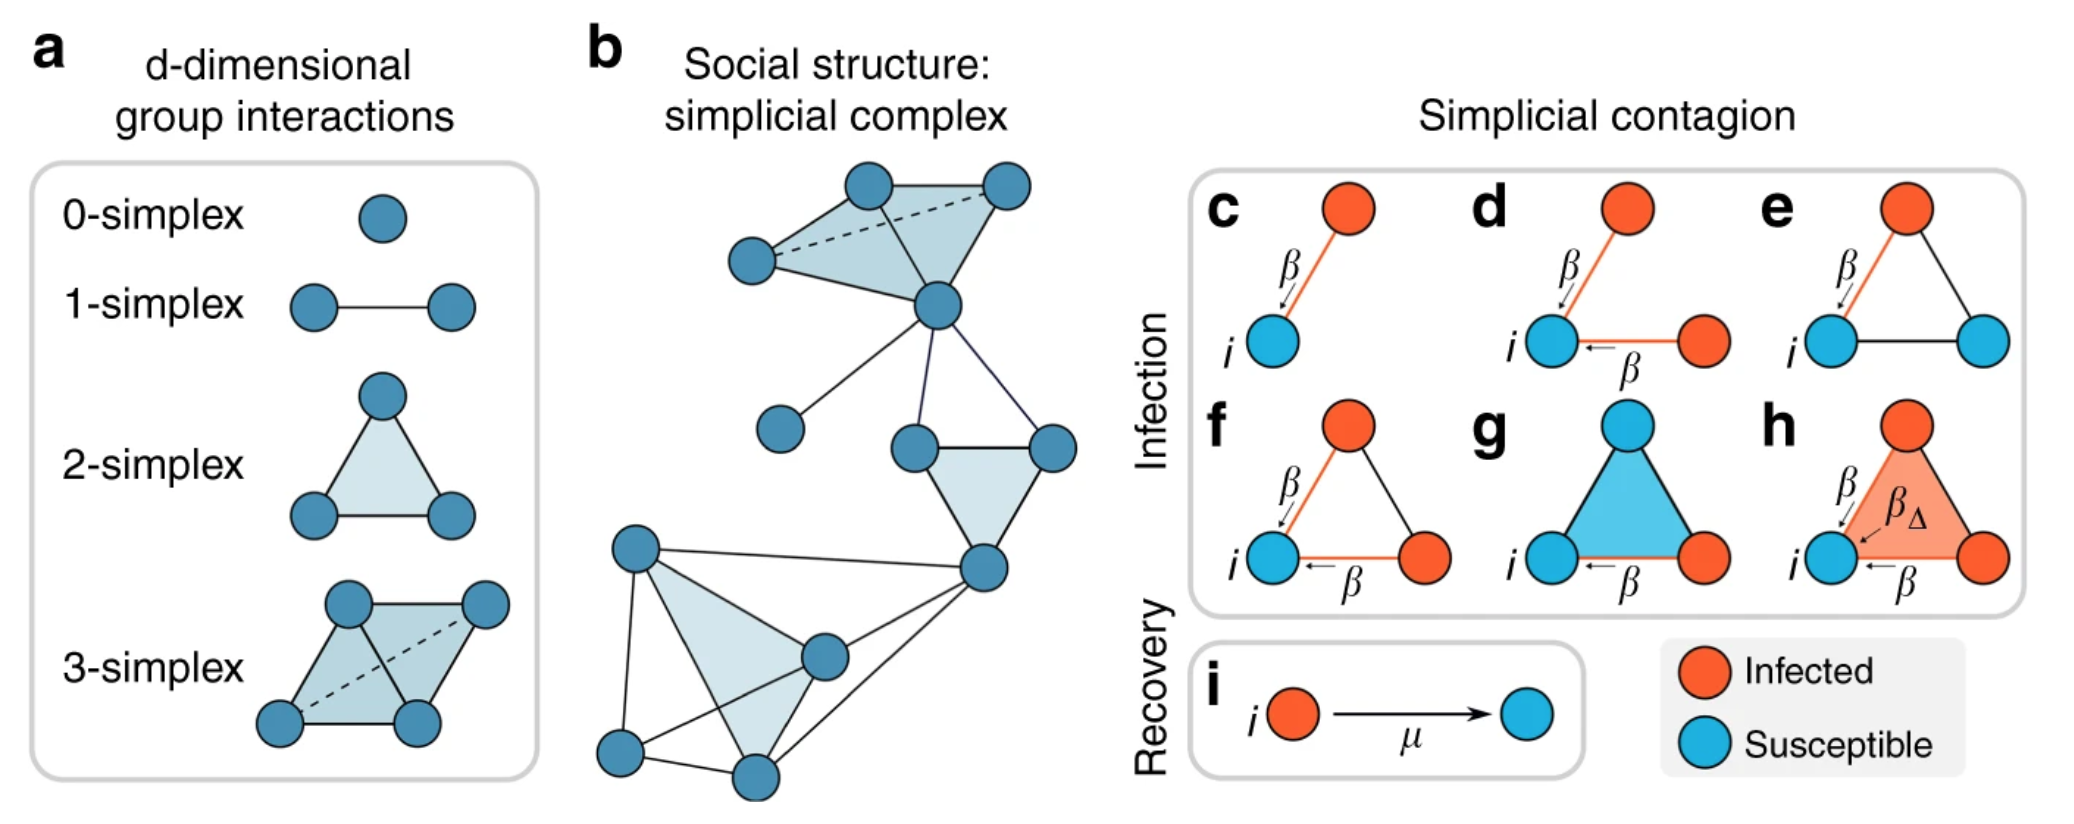
\includegraphics[width = 0.9\linewidth]{Pics/simplicial.png}
        \caption{Simplicial contagion model. \href{https://www.nature.com/articles/s41467-019-10431-6}{Source}}
        \label{fig:my_label}
    \end{figure}
\end{frame}

\begin{frame}{Q2: Function versus threats}
    \begin{figure}
        \begin{minipage}{0.48\linewidth}
            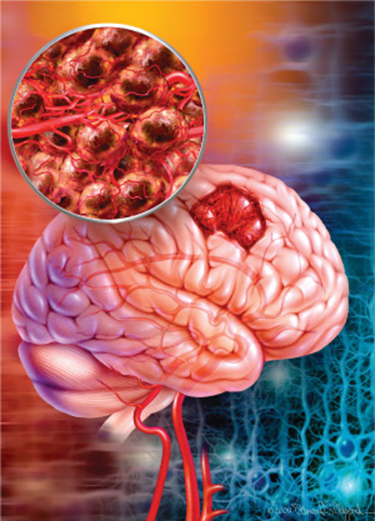
\includegraphics[width = 0.4\linewidth]{Pics/braintumor.jpg}
        \end{minipage}
        \begin{minipage}{0.48\linewidth}
            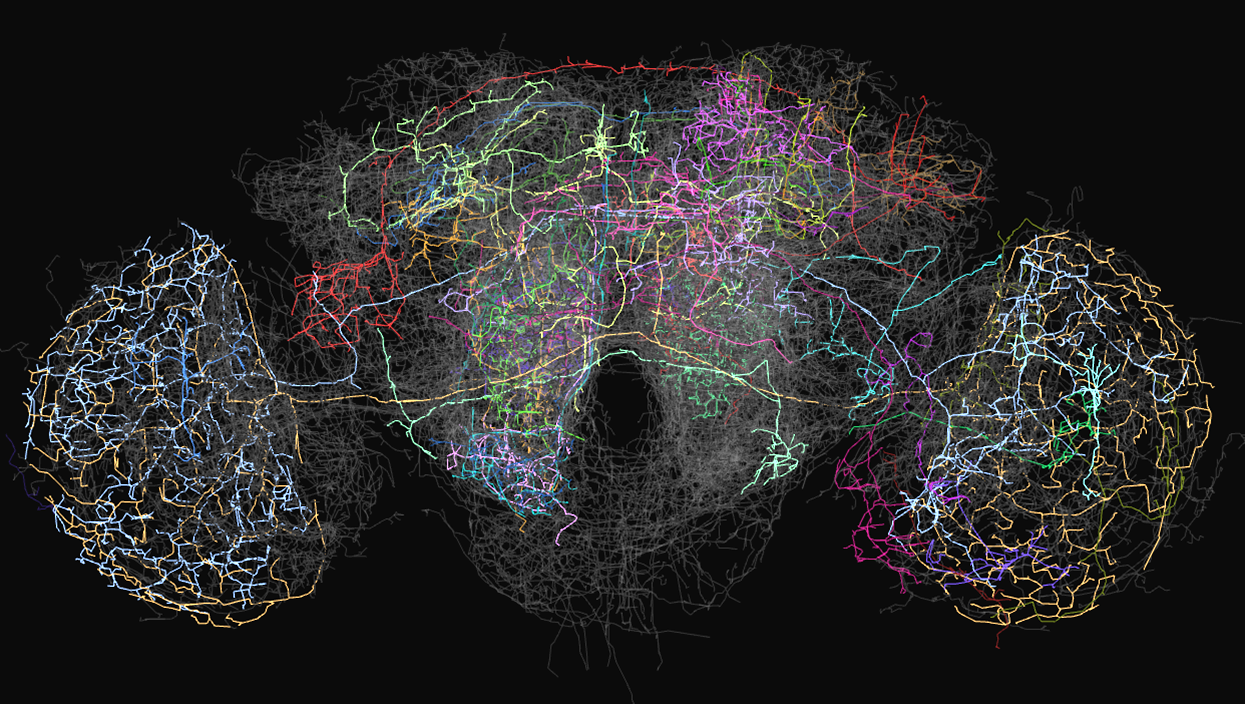
\includegraphics[width = 1\linewidth]{Pics/simple-words-about-the-complex-what-are-neural-networks-1.png}
        \end{minipage}
        \caption{Brain tumor (\href{http://medicalxtourism.com/wp-content/uploads/2014/06/Brain-Cancer-Symptoms-and-Tumor-Survival-Rate-in-UK.jpg}{\textit{source}}), and Neural network(\href{http://gadget.fsetyt.com/wp-content/uploads/2017/06/simple-words-about-the-complex-what-are-neural-networks-1.png}{\textit{source}}). It is interesting how functional organs, e.g., the brain, interconnects more topologically through links, such as synapsis or pipes; while the threat parts, such as tumors in brains and slums in cities, are usually spatial clusters.
        } 
    \end{figure}
    
\end{frame}


\begin{frame}{Q3: What's more?}
    \begin{center}
        \textbf{Let's find out together.}
    \end{center}
\end{frame}

\begin{frame}{Research plans: Timelines}
    \textbf{Timelines:} My visit will start from June or July. 
    \begin{center}
        \begin{tabular}	{|c|c|}
        \hline
        - to 2020-08 & Settle down, material reading,\\ & pick two/three projects \\ \hline
        2020-09 to 2020-10 & Basic experiments, discussions on \\ & values, feasibility, research proposals \\ \hline
        2020-11 to 2021-06 & Finish a work, revalue the aims below\\ \hline
        2021-07 to - & Collaborate on challenging topics\\ \hline 
        \end{tabular}
    \end{center}
    \textbf{Aims:} 
    \begin{itemize}
        \item (Hopefully) Find universal laws that exist both in human societies and microbial;
        \item Improve the theoretical basis of complex network theory;
        \item Give optimizations and solutions to cities with statistical physics.
    \end{itemize} 
\end{frame}